% Dibujo reutilizable; las etiquetas se definen en el tema que lo incluye.
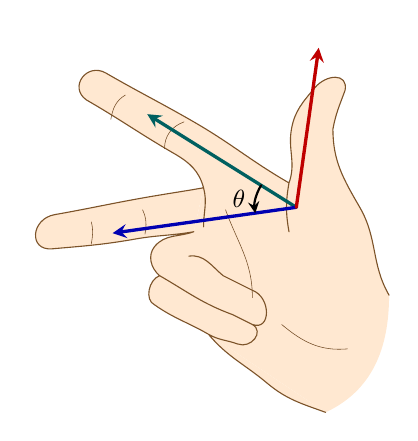
\begin{tikzpicture}[scale=.62,every node/.style={font=\small},>=stealth,
 line join=round,line cap=round]
\fill[orange!18] (2.9,-1.1)--(.85,1.2)--(-.9,1.1)--(-1.1,.2)
--(-1.8,-.7)--(-.8,-1.9)--(1.6,-3.5) to[out=25,in=-90] cycle;
\draw[fill=orange!18,draw=brown!65!black] (2.9,-1.1) to[out=120,in=-60] (2.3,.7) to[out=120,in=-90]
(1.75,2.3) to[out=80,in=-110] (2,3.1)
to[out=80,in=50,looseness=1.5] (1.38,3.15)
to[out=-130,in=80] (.9,2.3) to[out=-100,in=70] (.85,1.2)
to[out=-100,in=100] (.85,.2)
(.85,1.2) to[out=150,in=-30] (-1.1,2.45) to[out=150,in=-30] (-2.9,3.45)
to[out=150,in=145,looseness=1.7] (-3.3,2.9) to[out=-30,in=150] (-1.5,1.8)
to[out=-30,in=105] (-.9,1.1) to[out=-75,in=90] (-.9,.3)
(-.9,1.1) to[out=-170,in=10] (-2.1,.9) to[out=-170,in=10] (-3.95,.55)
to[out=-170,in=-175,looseness=1.8] (-4,-.15) to[out=5,in=-170] (-2.3,.05)
to[out=10,in=-170] (-1.1,.2)
(-1.1,.2) to[out=-160,in=50] (-1.9,-.1) to[out=-130,in=140] (-1.8,-.7)
to[out=-30,in=160] (-.3,-1.5)--(.1,-1.7)
to[out=-20,in=-20,looseness=1.5] (.1,-1)--(-.5,-.7) to[out=140,in=8] (-1.2,-.3)
(-1.8,-.7) to[out=-160,in=155] (-1.9,-1.3) to[out=-35,in=150] (-.8,-1.9)
to[out=-30,in=160] (-.2,-2.1) to[out=-20,in=-30,looseness=1.5] (.1,-1.7)
(-.8,-1.9) to[out=-50,in=140] (.4,-2.9) to[out=-40,in=160] (1.6,-3.5);
\draw[brown!60!black,very thin] (-1.3,2.45) to[out=-160,in=90] (-1.7,1.9)
(-2.5,3) to[out=-150,in=80] (-2.8,2.5)
(-2.1,.15) to[out=80,in=-65] (-2.15,.65)
(-3.2,-.05) to[out=80,in=-75] (-3.2,.4)
(-.45,.65) to[out=-70,in=90] (.1,-1.15)
(2.05,-2.2) to[out=-175,in=-40] (.7,-1.7);
\coordinate (O) at (1,.7);
\draw[->,very thick,teal!75!black] (O)--++(148:3.6) node[above left] {$\manoPrimero$};
\draw[->,very thick,blue!70!black] (O)--++(-172:3.8) node[left] {$\manoSegundo$};
\draw[->,very thick,red!75!black] (O)--++(82:3.3) node[above] {$\manoResultado$};
\draw[->,thick] (O)++(148:.85) arc(148:188:.85) node[midway,left] {$\theta$};
\end{tikzpicture}
